% ----------------------------------------------------------------
% AMS-LaTeX Paper ************************************************
% **** -----------------------------------------------------------
%\documentclass{amsart}
%\usepackage{txfonts}
%\documentclass[12pt,oneside]{article}
\documentclass{amsart}
\usepackage{graphicx}
\usepackage{enumitem}
% ----------------------------------------------------------------
\vfuzz2pt % Don't report over-full v-boxes if over-edge is small
\hfuzz2pt % Don't report over-full h-boxes if over-edge is small
% THEOREMS -------------------------------------------------------
\newtheorem{thm}{Theorem}[section]
\newtheorem{cor}[thm]{Corollary}
\newtheorem{lem}[thm]{Lemma}
\newtheorem{prop}[thm]{Proposition}
\theoremstyle{definition}
\newtheorem{defn}[thm]{Definition}
\theoremstyle{Exercise}
\newtheorem{ex}[thm]{Exercise}
\theoremstyle{remark}
\newtheorem{rem}[thm]{Remark}
\theoremstyle{rule}
\newtheorem{rul}[thm]{Rule}

\numberwithin{equation}{section}
% MATH -----------------------------------------------------------
\newcommand{\norm}[1]{\left\Vert#1\right\Vert}
\newcommand{\abs}[1]{\left\vert#1\right\vert}
\newcommand{\set}[1]{\left\{#1\right\}}
\newcommand{\Real}{\mathbb R}
\newcommand{\Z}{\mathbb Z}
\newcommand{\To}{\longrightarrow}
\newcommand{\BX}{\bB(X)}
\newcommand{\A}{\mathcal{A}}
% ----------------------------------------------------------------

% define some simple, commonly-used commands
\newcommand{\eps}{\varepsilon}
\newcommand{\dsum}{\displaystyle\sum}
\newcommand{\dint}{\displaystyle\int}

\newcommand{\pdr}[2]{\dfrac{\partial{#1}}{\partial{#2}}}
\newcommand{\pdrr}[2]{\dfrac{\partial^2{#1}}{\partial{#2}^2}}
\newcommand{\pdrt}[3]{\dfrac{\partial^2{#1}}{\partial{#2}{\partial{#3}}}}
\newcommand{\dr}[2]{\dfrac{d{#1}}{d{#2}}}
\newcommand{\aver}[1]{\langle {#1} \rangle}
\newcommand{\Baver}[1]{\Big\langle {#1} \Big\rangle}

\newcommand{\bzero}{\mathbf 0}
\newcommand{\bGamma}{\mbox{\boldmath{$\Gamma$}}}
\newcommand{\btheta}{\boldsymbol \theta}
\newcommand{\bchi}{\mbox{\boldmath{$\chi$}}}
\newcommand{\bnu}{\boldsymbol \nu}
\newcommand{\bmu}{\boldsymbol \mu}
\newcommand{\brho}{\mbox{\boldmath{$\rho$}}}
\newcommand{\bxi}{\boldsymbol \xi}
\newcommand{\bnabla}{\boldsymbol \nabla}
\newcommand{\bOm}{\boldsymbol \Omega}
\newcommand{\blambda}{\boldsymbol \lambda}
\newcommand{\bsigma}{\boldsymbol \sigma}

\newcommand{\bbR}{\mathbb R}
\newcommand{\bbC}{\mathbb C}
\newcommand{\bbQ}{\mathbb Q}
\newcommand{\bbN}{\mathbb N}
\newcommand{\bbZ}{\mathbb Z}

\newcommand{\ba}{\mathbf a} \newcommand{\bb}{\mathbf b}
\newcommand{\bc}{\mathbf c} \newcommand{\bd}{\mathbf d}
\newcommand{\be}{\mathbf e} \newcommand{\bff}{\mathbf f}
\newcommand{\bg}{\mathbf g} \newcommand{\bh}{\mathbf h}
\newcommand{\bi}{\mathbf i} \newcommand{\bj}{\mathbf j}
\newcommand{\bk}{\mathbf k} \newcommand{\bl}{\mathbf l}
\newcommand{\bm}{\mathbf m} \newcommand{\bn}{\mathbf n}
\newcommand{\bo}{\mathbf o} \newcommand{\bp}{\mathbf p}
\newcommand{\bq}{\mathbf q} \newcommand{\br}{\mathbf r}
\newcommand{\bs}{\mathbf s} \newcommand{\bt}{\mathbf t}
\newcommand{\bu}{\mathbf u} \newcommand{\bv}{\mathbf v}
\newcommand{\bw}{\mathbf w} \newcommand{\bx}{\mathbf x}
\newcommand{\by}{\mathbf y} \newcommand{\bz}{\mathbf z}
\newcommand{\bA}{\mathbf A} \newcommand{\bB}{\mathbf B}
\newcommand{\bC}{\mathbf C} \newcommand{\bD}{\mathbf D}
\newcommand{\bE}{\mathbf E} \newcommand{\bF}{\mathbf F}
\newcommand{\bG}{\mathbf G} \newcommand{\bH}{\mathbf H}
\newcommand{\bI}{\mathbf I} \newcommand{\bJ}{\mathbf J}
\newcommand{\bK}{\mathbf K} \newcommand{\bL}{\mathbf L}
\newcommand{\bM}{\mathbf M} \newcommand{\bN}{\mathbf N}
\newcommand{\bO}{\mathbf O} \newcommand{\bP}{\mathbf P}
\newcommand{\bQ}{\mathbf Q} \newcommand{\bR}{\mathbf R}
\newcommand{\bS}{\mathbf S} \newcommand{\bT}{\mathbf T}
\newcommand{\bU}{\mathbf U} \newcommand{\bV}{\mathbf V}
\newcommand{\bW}{\mathbf W} \newcommand{\bX}{\mathbf X}
\newcommand{\bY}{\mathbf Y} \newcommand{\bZ}{\mathbf Z}

\newcommand{\cA}{\mathcal A} \newcommand{\cB}{\mathcal B}
\newcommand{\cC}{\mathcal C} \newcommand{\cD}{\mathcal D}
\newcommand{\cE}{\mathcal E} \newcommand{\cF}{\mathcal F}
\newcommand{\cG}{\mathcal G} \newcommand{\cH}{\mathcal H}
\newcommand{\cI}{\mathcal I} \newcommand{\cJ}{\mathcal J}
\newcommand{\cK}{\mathcal K} \newcommand{\cL}{\mathcal L}
\newcommand{\cM}{\mathcal M} \newcommand{\cN}{\mathcal N}
\newcommand{\cO}{\mathcal O} \newcommand{\cP}{\mathcal P}
\newcommand{\cQ}{\mathcal Q} \newcommand{\cR}{\mathcal R}
\newcommand{\cS}{\mathcal S} \newcommand{\cT}{\mathcal T}
\newcommand{\cU}{\mathcal U} \newcommand{\cV}{\mathcal V}
\newcommand{\cW}{\mathcal W} \newcommand{\cX}{\mathcal X}
\newcommand{\cY}{\mathcal Y} \newcommand{\cZ}{\mathcal Z}


%%%%%%%%%%%%%%Start%%%%%%%%%%%%%Start%%%%%%%%%%%Start%%%%%%%%%%%%%%%Start%%%%%%%%%%%%%%%%%%%%%%%%%Start%%%%%%%%%%%%%%%%
%%%%%%%%%%%%%%Start%%%%%%%%%%%%%Start%%%%%%%%%%%Start%%%%%%%%%%%%%%%Start%%%%%%%%%%%%%%%%%%%%%%%%%Start%%%%%%%%%%%%%%%%
%%%%%%%%%%%%%%Start%%%%%%%%%%%%%Start%%%%%%%%%%%Start%%%%%%%%%%%%%%%Start%%%%%%%%%%%%%%%%%%%%%%%%%Start%%%%%%%%%%%%%%%%
\usepackage{xcolor}
\usepackage{fancyhdr}

\pagestyle{fancy}
\fancyhf{}
\rhead{}
\chead{\includegraphics[scale=.1]{snhu_logo.png}}

\begin{document}
\begin{center}
\includegraphics[scale=.1]{snhu_logo.png}
\end{center}
\title{\sf Module Five Problem Set}%


%\thm{bbjh}
\maketitle
This document is proprietary to Southern New Hampshire University. It and the problems within may not be posted on any non-SNHU website.\\\\\\\\
\begin{center}
%Enter your name below this line:
Ryan Hatch
\end{center}


\begin{center}
\rule{\textwidth}{0.4pt}
\end{center}


\newpage

%--------------------------------------------------------------------------------------------------
\section*{}
\section*{}
Directions: Type your solutions into this document and be sure to show all steps for arriving at your solution. Just giving a final number may not receive full credit.
\\\\
\section*{Problem 1}

Indicate whether the two functions are equal. If the two functions are not equal, then give an element of the domain on which the two functions have different values.\\
 \begin{enumerate}[label=(\alph*)]
   \item
\[ f: \Z \to \Z, \text{ where } f(x)= x^2.\]
\[ g: \Z \to \Z, \text{ where } g(x)= |x|^2.\]\\\\
%Enter your answer below this comment line.
The functions \( f \) and \( g \) defined are equal since for all \( x \in \mathbb{Z} \), \( x^2 = |x|^2 \).\\
Since the square of a real number is always a positive, and the square of an absolute value is also always a positive, for every integer $x$, I got $x^2 = |x|^2$. Considering that since squaring a number is equivalent to squaring its absolute value. Thus, the functions $f$ and $g$ are equal over their domain of all integers $\mathbb{Z}$.
\\\\
No element in the domain gives different values for $f$ and $g$, so the functions are equal.
\\\\
\item  \[ f: \Z\times \Z \to \Z, \text{ where } f(x,y)= |x+y|.\]
\[ g: \Z\times \Z \to \Z, \text{ where } g(x,y)= |x|+|y|.\]\\\\
%Enter your answer below this comment line.
The functions \( f \) and \( g \) defined are not equal. For \( x = -1 \) and \( y = 1 \), I found that \( f(-1,1) = 0 \) and \( g(-1,1) = 2 \), which shows that \( f(x,y) \neq g(x,y) \) for at least one element in the domain \( \mathbb{Z} \times \mathbb{Z} \).
\\\\
\end{enumerate}

 \newpage
%--------------------------------------------------------------------------------------------------

\section*{Problem 2}

The domain and target set of functions f and g is $\mathbb{R}$. The functions are defined as:
\begin{itemize}
  \item $f(x) = 2x + 3$\\

  \item $g(x) = 5x + 7$\\


\end{itemize}

\begin{enumerate}[label=(\alph*)]
\item  $f\circ g$?\\\\
%Enter your answer below this comment line.
To find \( f(g(x)) \), I substituted \( g(x) \) into \( f(x) \):
\[ f(g(x)) = f(5x + 7) = 2(5x + 7) + 3 = 10x + 14 + 3 = 10x + 17 \]
\\\\
\item  $g \circ f$?\\\\
%Enter your answer below this comment line.
To find \( g(f(x)) \), I substituted \( f(x) \) into \( g(x) \):
\[ g(f(x)) = g(2x + 3) = 5(2x + 3) + 7 = 10x + 15 + 7 = 10x + 22 \]
\\\\
\item  $(f\circ g)^{-1}$?\\\\
%Enter your answer below this comment line.
First, I had to find \( f \circ g \) as in part (a). The inverse function \( (f \circ g)^{-1} \) would undo the operation of \( f \circ g \), which is \( y = 10x + 17 \). Solving for \( x \) gave me:
\[ x = \frac{y - 17}{10} \]
So, \( (f \circ g)^{-1}(x) = \frac{x - 17}{10} \).
\\\\
\item  $f^{-1}\circ g^{-1}$?\\\\
%Enter your answer below this comment line.
First, I had to find the inverses of \( f \) and \( g \) separately:
\[ f^{-1}(x) = \frac{x - 3}{2} \quad \text{and} \quad g^{-1}(x) = \frac{x - 7}{5} \]
Then I calculated, \( f^{-1}(g^{-1}(x)) \):
\[ f^{-1}(g^{-1}(x)) = f^{-1}\left(\frac{x - 7}{5}\right) = \frac{\frac{x - 7}{5} - 3}{2} = \frac{x - 7 - 15}{10} = \frac{x - 22}{10} \]
\\\\
\item  $g^{-1}\circ f^{-1}$?\\\\
%Enter your answer below this comment line.
In a similar manner to earlier, I calculated, \( g^{-1}(f^{-1}(x)) \):
\[ g^{-1}(f^{-1}(x)) = g^{-1}\left(\frac{x - 3}{2}\right) = \frac{\frac{x - 3}{2} - 7}{5} = \frac{x - 3 - 14}{10} = \frac{x - 17}{10} \]
\\\\
\end{enumerate}
Are any of the above equal?\\\\
%Enter your answer below this comment line.
Upon comparing the expressions, I could see that \( (f \circ g)^{-1} \) from part (c) and \( g^{-1} \circ f^{-1} \) from part (e) are equal, as both simplify to \( \frac{x - 17}{10} \). None of the other compositions are equal to each other.
\\\\


    \newpage
%--------------------------------------------------------------------------------------------------



\section*{Problem 3}

\begin{enumerate}[label=(\alph*)]
\item  Give the matrix representation for the relation depicted in the arrow diagram. Then, express the relation as a set of ordered pairs.\\\\
The arrow diagram below represents a relation.\\
\fbox{
 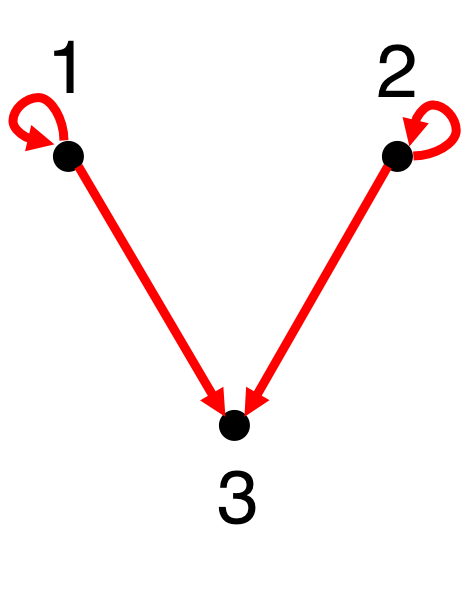
\includegraphics[width=2in]{M5-fig1}
}\\\\
{\color{blue}{\bf Figure 1:} \emph{An arrow diagram shows three vertices, 1, 2, and 3. An arrow from vertex 1 points to vertex 3, and another arrow from vertex 2 points to vertex 3. Two self loops are formed, one at vertex 1 and another at vertex 2. 
}
}
\\\\
%Enter your answer below this comment line.
%For more information on creating matrices in LaTeX, see this week's module resources.
The arrow diagram shows that there are three vertices (1, 2, and 3). A matrix representation will be a 3x3 matrix where the rows and columns represent the vertices. An entry of '1' in the matrix indicates a connection (or arrow) from the vertex represented by the row to the vertex represented by the column. A '0' indicates no connection. 

The self-loops at vertices 1 and 2 will be represented with '1's on the diagonal of the matrix. The connections from 1 to 3 and 2 to 3 will be represented with '1's in the appropriate positions.

The matrix representation \( M \) of the relation is:
\[
M = \begin{pmatrix}
1 & 0 & 1 \\
0 & 1 & 1 \\
0 & 0 & 0 \\
\end{pmatrix}
\]

And the relation \( R \) as a set of ordered pairs is:
\[ R = \{(1,1), (1,3), (2,2), (2,3)\} \]
\\

\item Draw the arrow diagram for the relation.\\
 The domain for the relation $A$ is the set $\{2,\, 5,\, 7,\, 8,\, 11\}$. For $x$, $y$ in the domain, $xAy$ if $|x-y|$ is less than $2$.
\\\\
%Enter your answer below this comment line.
To draw the arrow diagram for the relation \( A \), I  need to determine which elements in the domain have an absolute difference less than 2. We'll go through each pair in the domain:

- \( |2 - 5| = 3 \), so no arrow between 2 and 5.
- \( |2 - 7| = 5 \), so no arrow between 2 and 7.
- \( |2 - 8| = 6 \), so no arrow between 2 and 8.
- \( |2 - 11| = 9 \), so no arrow between 2 and 11.
- \( |5 - 7| = 2 \), so no arrow between 5 and 7 (since the difference is not less than 2).
- \( |5 - 8| = 3 \), so no arrow between 5 and 8.
- \( |5 - 11| = 6 \), so no arrow between 5 and 11.
- \( |7 - 8| = 1 \), so an arrow between 7 and 8.
- \( |7 - 11| = 4 \), so no arrow between 7 and 11.
- \( |8 - 11| = 3 \), so no arrow between 8 and 11.

The self-loops will occur for each element since \( |x - x| = 0 \), which is less than 2.
%To answer this question, you may hand-draw your solution or use a program like PowerPoint or Lucidchart.
%Take a photo or screenshot, then upload your file to this project. Note that the image you submit must be legible to your instructor.
%You will see your file name appear in the file tree. Uncomment the includegraphics line below and change the "YOURFILENAMEHERE" text to the name of the file that you uploaded. Your filename must match the name of your uploaded file.
%\includegraphics[width=2in]{YOURFILENAMEHERE} \\\\
\end{enumerate}
 \newpage
%--------------------------------------------------------------------------------------------------

\section*{Problem 4}

For each relation, indicate whether the relation is:
\begin{itemize}
  \item Reflexive, anti-reflexive, or neither
  \item Symmetric, anti-symmetric, or neither
  \item Transitive or not transitive
\end{itemize}
Justify your answer.\\
\begin{enumerate}[label=(\alph*)]
\item The domain of the relation $L$ is the set of all real numbers. For $x$, $y \in \Real, \; xLy$ if $x < y$.\\\\
%Enter your answer below this comment line.
The domain of the relation \( L \) is the set of all real numbers. \( xLy \) if \( x < y \).

Reflexive: A relation is reflexive if every element is related to itself. Since no real number is less than itself, the relation \( L \) is not reflexive.\\
Anti-Reflexive: A relation is anti-reflexive if no element is related to itself. Since \( x < x \) is never true, the relation \( L \) is anti-reflexive.\\
Symmetric: A relation is symmetric if whenever \( xLy \) then \( yLx \). Since if \( x < y \), it is not true that \( y < x \), the relation \( L \) is not symmetric.\\
Anti-Symmetric: A relation is anti-symmetric if whenever \( xLy \) and \( yLx \) are both true, then \( x = y \). This property does not apply here since \( xLy \) and \( yLx \) cannot both be true; thus, the relation \( L \) is anti-symmetric by definition.\\
Transitive: A relation is transitive if whenever \( xLy \) and \( yLz \), then \( xLz \). The relation \( L \) is transitive because if \( x < y \) and \( y < z \), then \( x < z \).
\\\\

\item The domain of the relation $A$ is the set of all real numbers. $xAy$ if $|x-y| \leq 2$\\\\
%Enter your answer below this comment line.
The domain of the relation \( A \) is the set of all real numbers. \( xAy \) if \( |x-y| \leq 2 \).

Reflexive: Since \( |x-x| = 0 \) which is less than or equal to 2, every number is related to itself, so the relation \( A \) is reflexive.\\
Symmetric: Since \( |x-y| \) is always equal to \( |y-x| \), if \( xAy \), then \( yAx \), so the relation \( A \) is symmetric.\\
Anti-Symmetric: The relation \( A \) is not anti-symmetric since there can be distinct \( x \) and \( y \) such that both \( xAy \) and \( yAx \) hold true without \( x = y \).\\
Transitive: The relation \( A \) is not necessarily transitive. For example, if \( x = 0 \), \( y = 2 \), and \( z = 4 \), then \( xAy \) and \( yAz \) but not \( xAz \) since \( |x-z| = 4 \) which is not less than or equal to 2.
\\\\
\item The domain of the relation $Z$ is the set of all real numbers. $xZy$ if $y=2x$\\\\\\\\
%Enter your answer below this comment line.
The domain of the relation \( Z \) is the set of all real numbers. \( xZy \) if \( y = 2x \).

Reflexive: The relation \( Z \) is not reflexive since for any real number \( x \), \( x \neq 2x \) (except for \( x = 0 \)).\\
Anti-Reflexive: The relation \( Z \) is not anti-reflexive because it relates \( 0 \) to itself since \( 0 = 2 \cdot 0 \).\\
Symmetric: The relation \( Z \) is not symmetric because if \( xZy \), there is no guarantee that \( yZx \) (for instance, \( 1Z2 \) but not \( 2Z1 \)).\\
Anti-Symmetric: The relation \( Z \) is anti-symmetric because if \( xZy \) and \( yZx \), then \( x = y \), which must hold true since the definition implies \( y = 2x \) and \( x = \frac{y}{2} \).\\
Transitive: The relation \( Z \) is transitive. If \( xZy \) and \( yZz \), then \( y = 2x \) and \( z = 2y \). Therefore, \( z = 4x \), and since \( z = 2(2x) \), it follows that \( xZ(2x) \) and \( (2x)Z(4x) \) implies \( xZ(4x) \).
\\\\
\end{enumerate}
\newpage
%--------------------------------------------------------------------------------------------------
\section*{Problem 5}

The number of watermelons in a truck are all weighed on a scale. The scale rounds the weight of every watermelon to the nearest pound. The number of pounds read off the scale for each watermelon is called its measured weight. The domain for each of the following relations below is the set of watermelons on the truck. For each relation, indicate whether the relation is:
\\
\begin{itemize}
  \item Reflexive, anti-reflexive, or neither
  \item Symmetric, anti-symmetric, or neither
  \item Transitive or not transitive
\end{itemize}
Justify your answer.\\

\begin{enumerate}[label=(\alph*)]
\item Watermelon $x$ is related to watermelon $y$ if the measured weight of watermelon $x$ is at least the measured weight of watermelon $y$. No two watermelons have the same measured weight.\\\\
%Enter your answer below this comment line.
Watermelon \( x \) is related to watermelon \( y \) if the measured weight of watermelon \( x \) is at least the measured weight of watermelon \( y \), and no two watermelons have the same measured weight.

Reflexive: The relation is not reflexive because no watermelon can have a measured weight that is at least as much as itself if all measured weights are unique.\\
Anti-Reflexive: The relation is anti-reflexive since no watermelon is related to itself due to the uniqueness of the measured weights.\\
Symmetric: The relation is not symmetric. If watermelon \( x \) is related to watermelon \( y \), meaning \( x \) weighs at least as much as \( y \), it does not imply that \( y \) weighs at least as much as \( x \) because no two watermelons can have the same measured weight.\\
Anti-Symmetric: The relation is anti-symmetric because if watermelon \( x \) is related to watermelon \( y \) and watermelon \( y \) is related to watermelon \( x \), then they would have to have the same measured weight, which is not possible as per the given condition.\\
Transitive: The relation is transitive. If watermelon \( x \) is related to watermelon \( y \) (meaning \( x \)'s weight is at least \( y \)'s), and \( y \) is related to watermelon \( z \), then \( x \) is also related to \( z \).\\
\\\\
\item Watermelon $x$ is related to watermelon $y$ if the measured weight of watermelon $x$ is at least the measured weight of watermelon $y$. All watermelons have exactly the same measured weight.\\\\
%Enter your answer below this comment line.
Watermelon \( x \) is related to watermelon \( y \) if the measured weight of watermelon \( x \) is at least the measured weight of watermelon \( y \), and all watermelons have exactly the same measured weight.

Reflexive: The relation is reflexive because every watermelon has a measured weight that is at least as much as itself, as all measured weights are the same.\\
Anti-Reflexive: The relation is not anti-reflexive since every watermelon is related to itself.\\
Symmetric: The relation is symmetric because if watermelon \( x \) is related to watermelon \( y \), then \( y \) is also related to \( x \), as their measured weights are the same.\\
Anti-Symmetric: The relation is not anti-symmetric in this scenario because even though watermelon \( x \) is related to watermelon \( y \) and \( y \) is related to \( x \), they are not the same watermelon, yet their measured weights are equal.\\
Transitive: The relation is transitive because if watermelon \( x \) is related to watermelon \( y \), and \( y \) is related to watermelon \( z \), then \( x \) is also related to \( z \) since all their measured weights are the same.
\\\\
\end{enumerate}
 \newpage
%--------------------------------------------------------------------------------------------------

\section*{Problem 6}
\subsection*{Part 1}
Give the adjacency matrix for the graph G as pictured below:\\
\\
\fbox{
 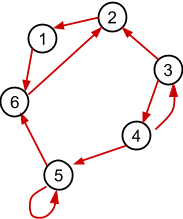
\includegraphics[width=1.75in]{M5-fig2}\\
}\\\\
{\color{blue}{\bf Figure 2:} \emph{A graph shows 6 vertices and 9 edges. The vertices are 1, 2, 3, 4, 5, and 6, represented by circles. The edges between the vertices are represented by arrows, as follows: 4 to 3; 3 to 2; 2 to 1; 1 to 6; 6 to 2; 3 to 4; 4 to 5; 5 to 6; and a self loop on vertex 5.
}
}\\
%Enter your answer below this comment line.
%For more information on creating matrices in LaTeX, see this week's module resources.
The adjacency matrix for a directed graph is a square matrix where each element \( a_{ij} \) is \( 1 \) if there is an edge from vertex \( i \) to vertex \( j \), and \( 0 \) otherwise.\\

Vertex 1 has an edge to vertex 6.\\
Vertex 2 has an edge to vertex 1.\\
Vertex 3 has edges to vertices 2 and 4.\\
Vertex 4 has edges to vertices 3 and 5.\\
Vertex 5 has a self-loop and an edge to vertex 6.\\
Vertex 6 has an edge to vertex 2.\\

The adjacency matrix \( A \) for graph G is:

\[
A  = \begin{pmatrix}
0 & 0 & 0 & 0 & 0 & 1 \\
1 & 0 & 0 & 0 & 0 & 0 \\
0 & 1 & 0 & 1 & 0 & 0 \\
0 & 0 & 1 & 0 & 1 & 0 \\
0 & 0 & 0 & 0 & 1 & 1 \\
0 & 1 & 0 & 0 & 0 & 0 \\
\end{pmatrix}
\]
\\\\

\subsection*{Part 2}
A directed graph $G$ has 5 vertices, numbered 1 through 5. The $5\times 5$ matrix $A$ is the adjacency matrix for $G$. The matrices $A^2$ and $A^3$ are given below.
\[
A^2  = \left( \begin{array}{ccccc}
0 & 1 & 0 & 0 & 0 \\
0 & 0 & 1 & 0 & 0\\
1 & 0 & 0 & 0 & 0\\
1 & 0 & 0 & 1 & 0\\
0 & 1 & 1 & 0 & 1
\end{array} \right)~~~~~~~
\]
\[
A^3  = \left( \begin{array}{ccccc}
1 & 0 & 0 & 0 & 0 \\
0 & 1 & 0 & 0 & 0\\
0 & 0 & 1 & 0 & 0\\
0 & 1 & 1 & 0 & 1\\
1 & 1 & 0 & 1 & 0
\end{array} \right)~~~~~~~
\]
Use the information given to answer the questions about the graph G.
\begin{enumerate}[label=(\alph*)]
\item Which vertices can reach vertex 2 by a walk of length 3?\\\\
%Enter your answer below this comment line.
To determine which vertices can reach vertex 2 by a walk of length 3, I looked at the third power of the adjacency matrix \( A^3 \), specifically at the column corresponding to vertex 2. The non-zero entries in this column indicate vertices that can reach vertex 2 in 3 steps.

From the matrix \( A^3 \), I noted that the vertices that can reach vertex 2 by a walk of length 3 are vertices 1, 5, and 6 (since the first, fifth, and sixth rows in the second column of \( A^3 \) have non-zero entries).
\\\\

\item Is there a walk of length 4 from vertex 4 to vertex 5 in $G$? (Hint: $A^4 = A^2\cdot A^2$.)\\\\
%Enter your answer below this comment line.
To find out if there is a walk of length 4 from vertex 4 to vertex 5, I had to calculate the fourth power of the adjacency matrix \( A^4 \) (or simply square the matrix \( A^2 \)). I was interested in the element in the fourth row and fifth column of \( A^4 \), which would tell me if there is a walk of length 4 from vertex 4 to vertex 5.

Since the hint suggests \( A^4 = A^2 \cdot A^2 \), I multiplied \( A^2 \) by itself:

\[
A^2  = \begin{pmatrix}
0 & 1 & 0 & 0 & 0 \\
0 & 0 & 1 & 0 & 0 \\
1 & 0 & 0 & 0 & 0 \\
1 & 0 & 0 & 1 & 0 \\
0 & 1 & 1 & 0 & 1 \\
\end{pmatrix} \times 
\begin{pmatrix}
0 & 1 & 0 & 0 & 0 \\
0 & 0 & 1 & 0 & 0 \\
1 & 0 & 0 & 0 & 0 \\
1 & 0 & 0 & 1 & 0 \\
0 & 1 & 1 & 0 & 1 \\
\end{pmatrix} 
\]

The product gave me, \( A^4 \), and I could then check the element in the fourth row and fifth column to answer the question. If the result in that position is non-zero, it means there is at least one walk of length 4 from vertex 4 to vertex 5.
The matrix \( A^4 \) is calculated as follows:

\[
A^4  = \begin{pmatrix}
0 & 0 & 1 & 0 & 0 \\
1 & 0 & 0 & 0 & 0 \\
0 & 1 & 0 & 0 & 0 \\
1 & 1 & 0 & 1 & 0 \\
1 & 1 & 2 & 0 & 1 \\
\end{pmatrix}
\]

From the matrix \( A^4 \), I looked at the entry in the fourth row and fifth column to determine if there is a walk of length 4 from vertex 4 to vertex 5. Since this entry is 0, there is no walk of length 4 from vertex 4 to vertex 5 in the graph \( G \).

\end{enumerate}

 \newpage
%--------------------------------------------------------------------------------------------------

\section*{Problem 7}
\subsection*{Part 1} The drawing below shows a Hasse diagram for a partial order on the set $\{A,\, B,\, C,\, D,\, E,\, F,\, G,\, H,\, I,\, J\}$
\\
\\
\fbox{
 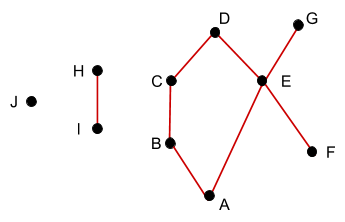
\includegraphics[width=2in]{M5-fig3}\\
}\\
\\
{\color{blue}{\bf Figure 3:} \emph{A Hasse diagram shows 10 vertices and 8 edges. The vertices, represented by dots, are as follows: vertex J; vertices H and I are aligned vertically to the right of vertex J; vertices A, B, C, D, and E forms a closed loop, which is to the right of vertices H and I; vertex G is inclined upward to the right of vertex E; and vertex F is inclined downward to the right of vertex E. The edges, represented by line segments, between the vertices are as follows: Vertex J is connected to no vertex; a vertical edge connects vertices H and I; a vertical edge connects vertices B and C; and 6 inclined edges connect the following vertices, A and B, C and D, D and E, A and E, E and G, and E and F.
}
}
\\
\\

\begin{enumerate}[label=(\alph*)]
\item What are the minimal elements of the partial order?\\\\
%Enter your answer below this comment line.
Minimal elements are those that have no elements below them. In the Hasse diagram, these are the elements with no edges coming into them from below. Based on Figure 3, the minimal elements of the partial order are A, J, and I.
\\\\

\item What are the maximal elements of the partial order?\\\\
%Enter your answer below this comment line.
Maximal elements are those that have no elements above them. In the Hasse diagram, these are the elements with no edges going out from them to above. Based on Figure 3, the maximal elements of the partial order are H, G, and F.
\\\\

\item Which of the following pairs are comparable?\\
\[
(A, \,D),\, (J,\, F),\, (B,\, E),\, (G, \,F),\, (D,\, B),\, (C, \,F),\, (H,\, I), \,(C,\, E)
\]\\\\
%Enter your answer below this comment line.
Two elements are comparable if there is a path (following the direction of the edges) from one to the other. For the pairs given:

- \( (A, D) \): Comparable, since there's a path A to E to D.
- \( (J, F) \): Not comparable, J is isolated.
- \( (B, E) \): Comparable, since there's a path B to C to D to E.
- \( (G, F) \): Not comparable, there are no paths between G and F.
- \( (D, B) \): Not comparable, since the direction B to D is not followed.
- \( (C, F) \): Not comparable, there are no paths from C to F.
- \( (H, I) \): Comparable, since there's a path from I to H.
- \( (C, E) \): Comparable, since there's a path from C to D to E.
\\\\

\end{enumerate}

\subsection*{Part 2}
Each relation given below is a partial order. Draw the Hasse diagram for the partial order.

\begin{enumerate}[label=(\alph*)]
\item The domain is $\{3,\, 5,\, 6,\, 7,\, 10,\, 14,\, 20,\, 30,\, 60\}$. $x \leq y$ if $x$ evenly divides $y$.\\\\
%Enter your answer below this comment line.

%To answer this question, you may hand-draw your solution or use a program like PowerPoint or Lucidchart.
%Take a photo or screenshot, then upload your file to this project. Note that the image you submit must be legible to your instructor.
%You will see your file name appear in the file tree. Uncomment the includegraphics line below and change the "YOURFILENAMEHERE" text to name of the file that you uploaded. Your filename must match the name of your uploaded file.
\includegraphics[width=2in]{problem7a.jpeg}\\\\

\item The domain is $\{a,\, b,\, c,\, d,\, e,\, f\}$. The relation is the set:
\[
\{ (b,\, e),\, (b,\, d),\, (c,\, a),\, (c,\, f),\, (a,\, f),\, (a,\, a),\, (b,\, b),\, (c, \,c),\, (d,\, d),\, (e, \,e), \,(f,\, f) \}
\]\\\\
%Enter your answer below this comment line.

%To answer this question, you may hand-draw your solution or use a program like PowerPoint or Lucidchart.
%Take a photo or screenshot, then upload your file to this project. Note that the image you submit must be legible to your instructor.
%You will see your file name appear in the file tree. Uncomment the includegraphics line below and change the "YOURFILENAMEHERE" text to name of the file that you uploaded. Your filename must match the name of your uploaded file.
\includegraphics[width=2in]{problem7b.jpeg}\\\\

\end{enumerate}

\newpage%--------------------------------------------------------------------------------------------------

\section*{Problem 8}

Determine whether each relation is an equivalence relation. Justify your answer. If the relation is an equivalence relation, then describe the partition defined by the equivalence classes.\\
\begin{enumerate}[label=(\alph*)]
\item The domain is a group of people. Person $x$ is related to person $y$ under relation $M$ if $x$ and $y$ have the same favorite color. You can assume that there is at least one pair in the group, $x$ and $y$, such that $xMy$.\\\\
%Enter your answer below this comment line.
Relation \( M \) in a group of people where person \( x \) is related to person \( y \) if they have the same favorite color.

Reflexive: Every person has the same favorite color as themselves, so the relation is reflexive.\\
Symmetric: If person \( x \) has the same favorite color as person \( y \), then person \( y \) has the same favorite color as person \( x \), so the relation is symmetric.\\
Transitive: If person \( x \) has the same favorite color as person \( y \), and person \( y \) has the same favorite color as person \( z \), then person \( x \) has the same favorite color as person \( z \), so the relation is transitive.\\

Since the relation \( M \) is reflexive, symmetric, and transitive, it is an equivalence relation.

The partition defined by the equivalence classes would consist of subsets of people, where all members of a subset have the same favorite color. Each subset would be mutually exclusive, meaning no person belongs to more than one subset, and collectively exhaustive, meaning every person in the group belongs to one subset.
\\\\

\item The domain is the set of all integers. $xEy$ if $x + y$ is even. An integer $z$ is even if $z = 2k$ for some integer $k$.\\\\
%Enter your answer below this comment line.
Relation \( E \) in the set of all integers where \( xEy \) if \( x + y \) is even.

Reflexive: This relation is not reflexive. For an integer \( x \), \( x + x = 2x \) is always even, which would suggest reflexivity. However, for reflexivity, \( xEx \) must hold for all \( x \), and the relation defined as \( x + y \) being even does not allow me to confirm \( xEx \) without considering \( y \).\\
Symmetric: The relation is symmetric. If \( xEy \) (meaning \( x + y \) is even), then \( yEx \) (since \( y + x \) is also even, as addition is commutative).\\
Transitive: The relation is not transitive. For example, if \( x = 1 \), \( y = 1 \), and \( z = 2 \), then \( xEy \) and \( yEz \) (since \( 1 + 1 \) and \( 1 + 2 \) are even), but \( xEz \) does not hold since \( 1 + 2 \) is not even.

Since the relation \( E \) is symmetric but not reflexive nor transitive, it is not an equivalence relation. Therefore, it does not define a partition into equivalence classes.
\\\\

\end{enumerate}
%--------------------------------------------------------------------------------------------------



\end{document}
